%
% File emnlp2020.tex
%
%% Based on the style files for ACL 2020, which were
%% Based on the style files for ACL 2018, NAACL 2018/19, which were
%% Based on the style files for ACL-2015, with some improvements
%%  taken from the NAACL-2016 style
%% Based on the style files for ACL-2014, which were, in turn,
%% based on ACL-2013, ACL-2012, ACL-2011, ACL-2010, ACL-IJCNLP-2009,
%% EACL-2009, IJCNLP-2008...
%% Based on the style files for EACL 2006 by 
%%e.agirre@ehu.es or Sergi.Balari@uab.es
%% and that of ACL 08 by Joakim Nivre and Noah Smith

\documentclass[11pt,a4paper]{article}
\usepackage[hyperref]{emnlp2020}
\usepackage{times}
\usepackage{latexsym}
\renewcommand{\UrlFont}{\ttfamily\small}

% This is not strictly necessary, and may be commented out,
% but it will improve the layout of the manuscript,
% and will typically save some space.
\usepackage{microtype}

\usepackage{mystyle}
\usepackage{subcaption} 

% trellis
\usepackage{tikz}%

\usepackage{algorithm}
\usepackage[noend]{algpseudocode}

\usepackage{pgfplots}

%% ADD BACK!!!!!!!!!!!!!!!!!
\aclfinalcopy % Uncomment this line for the final submission
\def\aclpaperid{3272} %  Enter the acl Paper ID here

%\setlength\titlebox{5cm}
% You can expand the titlebox if you need extra space
% to show all the authors. Please do not make the titlebox
% smaller than 5cm (the original size); we will check this
% in the camera-ready version and ask you to change it back.

\newcommand\BibTeX{B\textsc{ib}\TeX}
\newcommand\Emit{\mathbf{O}}
\newcommand\Trans{\mathbf{T}}

\title{Scaling Hidden Markov Language Models}

\author{Justin T. Chiu {\normalfont and} Alexander M. Rush\\
  Department of Computer Science \\
  Cornell Tech \\
  \texttt{\{jtc257,arush\}@cornell.edu}\\}
%\And
  %Alexander M. Rush \\
  %Department of Computer Science \\
  %Cornell Tech \\
  %\texttt{arush@cornell.edu} \\}

\date{}

\begin{document}
\maketitle
\begin{abstract}
The hidden Markov model (HMM) is a fundamental tool for sequence modeling that 
cleanly separates the hidden state from the emission structure.
However, this separation makes it difficult to fit HMMs to large datasets in modern NLP, 
and they have fallen out of use due to very poor performance 
compared to fully observed models. This work revisits the challenge of 
scaling HMMs to language modeling datasets,
taking ideas from recent approaches to neural modeling.
We propose methods for scaling HMMs to massive state spaces
while maintaining efficient exact inference, a compact parameterization,
and effective regularization.
Experiments show that this approach leads to models that are much more accurate
than previous HMMs and n-gram-based methods,
making progress towards the performance of state-of-the-art neural models.
\end{abstract}

\section{Introduction}

Hidden Markov models (HMMs) are a fundamental latent-variable model for sequential data,
with a rich history in NLP.
They have been used extensively in NLP tasks such as
tagging \citep{merialdo1994tagging}, alignment \citep{vogel1996hmm},
and even, in a few cases, language modeling \citep{kuhn1994hmmlm,huang2011thesis}. 
Compared to other sequence models, HMMs are naturally appealing since they 
fully separate the process of generating hidden states from observations,
while allowing for exact posterior inference. 

State-of-the-art systems in NLP have moved away from utilizing latent hidden states
and toward deterministic deep neural models.
We take several lessons from the success of neural models for NLP tasks:
(a) model size is critical for accuracy,
e.g. large LSTMs \cite{zaremba2014lstm} show marked improvements in performance;
(b) the right factorization is critically important for representation learning,
e.g. a feedforward model \cite{bengio2003nlm}
can have the same probabilistic structure as an n-gram model while performing significantly better;
(c) dropout is key to achieving strong performance \citep{zaremba2014lstm,merity2017awdlstm}.

We revisit HMMs for language modeling,
positing that competitive performance may require very large models. 
Our contributions are as follows:
We demonstrate large improvements in an HMM language model by scaling the state space.
Towards that goal, we introduce three techniques:
a modeling constraint that allows us to use a large number of states 
while maintaining efficient exact inference,
a neural parameterization that improves
generalization while remaining faithful to the
probabilistic structure of the HMM,
and a variant of dropout that both improves accuracy
and halves the computational overhead during training. 

Experiments employ HMMs on two language modeling datasets.
Our three techniques allow us to train an HMM with tens of thousands of states,
significantly outperforming past HMMs as well as n-gram models.

\section{Related Work}
\label{sec:rw}
In order to improve the performance of HMMs on language modeling,
several recent papers have combined HMMs with neural networks.
\citet{buys2018hmm} develop an approach to relax HMMs,
but their models either perform poorly or alters the probabilistic structure to resemble an RNN. 
\citet{krakovna2016hmm} utilize model combination with an RNN to connect both approaches in a
20 state model.
We instead improve pure HMMs by scaling to many states.

% Prior work has tried neural parameterizations, but with small state spaces.
Prior work has considered neural parameterizations of HMMs. 
\citet{tran2016hmm} demonstrate improvements in POS induction with a
neural parameterization of an HMM.
They consider small state spaces,
as the goal was tag induction rather than language modeling.\footnote{
Other work has used neural parameterization for structured models, such as 
dependency models \citep{han2017dependency},
hidden semi-Markov models \citep{wiseman2018hsmm},
and context free grammars \citep{kim2019cpcfg}.
}

% Prior work has tried large state spaces with scalar parameterizations.
Prior work has also used HMMs with many states.
\citet{dedieu2019learning} introduce a sparsity constraint
in order to train a 30K state non-neural HMM for character-level language modeling;
however, their constraint precludes application to large vocabularies.
We overcome this limitation and train models with 
neural parameterizations on word-level language modeling.

% State splitting / refinement
Finally, another approach for scaling state spaces is to
grow from small to big via a split-merge process
\citep{petrov2006splitmerge,huang2011thesis}.
In particular, \citet{huang2011thesis} learn an HMM for language modeling
via this process.
As fixed-size state spaces are amenable to batching GPU,
we leave split-merge procedures for future work. 

\section{Background: HMMs}

We are interested in learning a distribution over observed tokens
$\bx = \langle x_1, \ldots, x_T \rangle$, with each token $x_t$
an element of the finite vocabulary $\mcX$.
Hidden Markov models (HMMs) specify a joint distribution over 
observed tokens $\bx$ and discrete latent states $\bz = \langle z_1, \ldots, z_T \rangle$,
with each $z_t$ from the finite set $\mcZ$.
For notational convenience, we define the starting state $z_0=\epsilon$.
This yields the joint distribution
\begin{equation}
p(\bx, \bz; \theta)
= \prod_{t=1}^T p(x_t\mid z_t)p(z_t \mid z_{t-1})
\end{equation}
\noindent The distributions are parameterized as follows
\begin{equation}
\label{param}
%p(z_1 | z_0) &\propto e^{\psi_{z_1}}\\
p(z_t \mid z_{t-1}) \propto e^{\psi_{z_{t-1}z_t}} \quad \ p(x_t \mid z_t) \propto e^{\phi_{z_tx_t}}
\end{equation}
with transitions $\psi \in \mathbb{R}^{|\mcZ|\times|\mcZ|}$
and emissions $\phi \in \mathbb{R}^{|\mcZ| \times |\mcX|}$.
These are the distributional parameters of an HMM,
and we refer to the emission matrix with entries $p(x_t \mid z_t)$ as $\mathbf{O}$.

We distinguish between two types of model parameterizations: \textit{scalar} and \textit{neural},
where the model parameters are given by $\theta$.
A scalar parameterization sets the model parameters equal to the distributional
parameters, so that $\theta = \set{\phi,\psi}$,
resulting in $O(|\mcZ|^2 + |\mcZ||\mcX|)$ model parameters.
A neural parameterization instead generates the distributional parameters
from a neural network (with parameters $\theta$),
decoupling the size of $\theta$ from $\phi,\psi$.
This decoupling gives us the ability to choose
between compact or overparameterized $\theta$ (relative to $\phi,\psi$).
As we will use large state spaces,
we take advantage of compact neural parameterizations.

In order to fit an HMM to data $\bx$,
we must marginalize over the latent states to obtain the likelihood
$p(\bx) = \sum_{\bz}p(\bx,\bz)$.
This sum can be computed in time $O(T|\mcZ|^2)$ via the forward algorithm,
which becomes prohibitive if the number of latent states $|\mcZ|$ is large.
We can then optimize the likelihood 
with gradient ascent (or alternative variants of expectation maximization).
See the appendix for more details on inference and optimization in HMMs.

\noindent \textbf{HMMs and RNNs}
Although the forward algorithm resembles that of the forward pass in a recurrent neural network (RNN)
\citep{buys2018hmm}, there are key representational differences.
RNNs do not decouple the latent dynamics from the observed.
This often leads to improved accuracy,
but precludes posterior inference which is useful for interpretability.
A further benefit of HMMs over RNNs is that
their associative structure allows for parallel inference
via the prefix-sum algorithm \cite{ladner1980prefix}.\footnote{
Quasi-RNNs \citep{bradbury2016qrnn} also have a logarithmic dependency on $T$
by applying the same prefix-sum trick, but do not model uncertainty over
latent dynamics.}
Finally, HMMs bottleneck information from every timestep through a discrete hidden state. 
NLP has a long history of utilizing discrete representations,
and returning to explore discrete representations may yield interesting results.
For example, recent work has found that discrete latent variables
work well in low-resource regimes \citep{jin2020discrete}.


\section{Scaling HMMs}
\label{sec:methods}

\begin{figure}[t]
\centering
%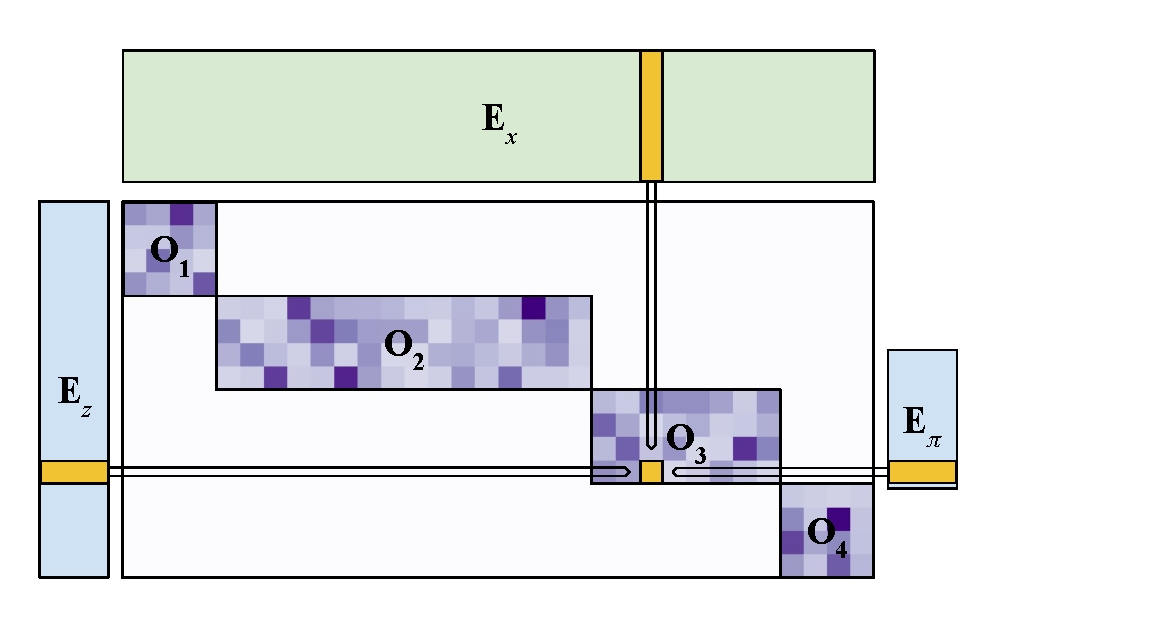
\includegraphics[height=1.7in]{img/mat.pdf}
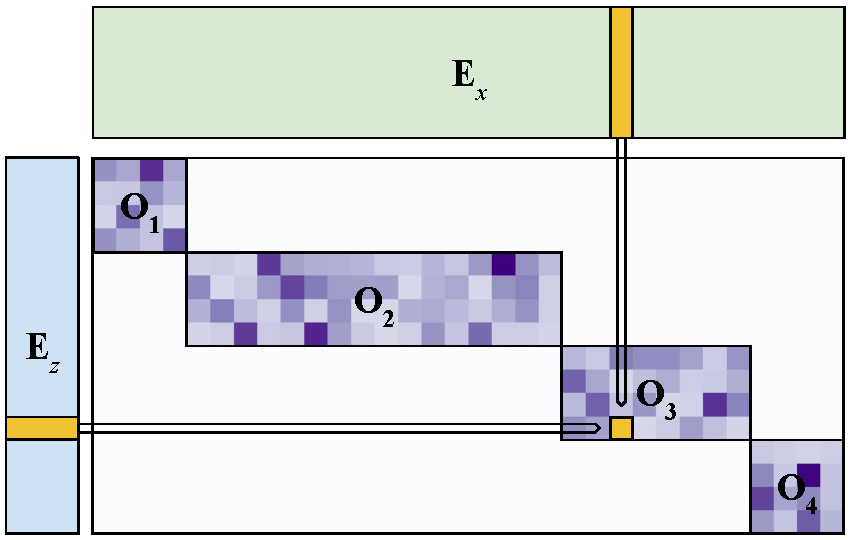
\includegraphics[height=1.7in]{img/blocksparse_mat_no_block.pdf}
\caption{\label{fig:emit}
The emission matrix as a set of blocks $\mathbf{O}_1, \ldots, \mathbf{O}_4$
with fixed height $k$.
The width of each block may vary, as there is no constraint on the number of words
a state can emit.
Each active cell is constructed from word $\mathbf{E}_x$ and state $\mathbf{E}_z$
embeddings.
}
\end{figure}

\noindent
\textbf{Blocked Emissions} Efficiency of marginal inference inherently limits 
the state space of general HMMs.
However, we can improve inference complexity in special cases.
As states in an HMM are used to represent context, a reasonable assumption
is that not every word should be used in every context.
Inspired by cloned HMMs \citep{dedieu2019learning},
we constrain our HMMs to have rectangular blocked emissions,
\[\mathbf{O} = \begin{bmatrix} \mathbf{O}_1 & 0 & 0 \\ 0 & $\dots$ & 0 \\ 0 & 0 & \mathbf{O}_M \\
\end{bmatrix}\]
where each $\mathbf{O}_m \in \mathbb{R}^{ k \times |\mcX_m|}$ ($k = |{\mcZ}|/M$)
is a partition indicating which tokens $\mcX_m$ can be emitted by states
$mk$ through $(m+1)k$.
Conversely, let $\mcZ_x \subset {\cal Z}$ be the states with non-zero probability of emitting $x$
(with $|\mcZ_x| = k$).
Exact marginalization can be computed via 
\begin{equation}
\label{eqn:sparse_marginalization}
\begin{aligned}
p(\bx) &= \sum_{z_1 \in \mcZ_{x_1}} p(z_1\mid z_0)p(x_1 \mid z_1) \times\\
    &\cdots
    \sum_{z_T \in \mcZ_{x_T}} p(z_T \mid z_{T-1})p(x_T \mid z_T)
\end{aligned}
\end{equation}
Since there are only $k$ states with nonzero probability of occurring
at every timestep, we only need to consider transitioning from the $|\mcZ_{x_t}| = k$
previous states to the next $|\mcZ_{x_{t+1}}|=k$ states,
resulting in $O(k^2)$ operations per timestep.
This gives a serial complexity of $O(Tk^2)$.\footnote{
This can be sped up on a parallel machine to $O(\log(T)k^2)$
via a binary reduction.
}

\vspace{0.2cm}

\noindent
\textbf{Neural Parameterization}
Even with blocked emissions, the scalar parameterization of an HMM grows as $O(|\mcZ|^2)$.
We instead employ a neural parameterization.
The approach is to embed each state in $\mcZ$ ($\mathbf{E}_z \in \mathbb{R}^{|\mcZ| \times h}$)
and each token in $\cal X$ ($\mathbf{E}_x \in \mathbb{R}^{|\mcX| \times h}$).
From these we can create representations for leaving and entering a state,
and emitting a word: 
\[ \mathbf{H}_{\textrm{out}},\mathbf{H}_{\textrm{in}},\mathbf{H}_\textrm{emit}
 = \text{MLP}( \mathbf{E}_z ) \] 
with all $\mathbf{H}_{\bullet} \in \mathbb{R}^{|\mcZ|\times h}$.
The HMM distributional parameters are given by
\begin{equation}
\begin{aligned}
\phi = \mathbf{H}_\textrm{emit}\mathbf{E}_x ^\top \qquad 
\psi = \mathbf{H}_\textrm{in}\mathbf{H}_\textrm{out}^\top
\end{aligned}
\end{equation}
where $\phi \in \mathbb{R}^{|\mcZ|\times|\mcX|}$ and
$\psi \in \mathbb{R}^{|\mcZ|\times|\mcZ|}$.
The MLP architecture follows \cite{kim2019cpcfg}, with details in the appendix.
This neural parameterization takes $O(h^2 + h|\mcZ| + h|\mcX|)$ parameters
(shown in Figure~\ref{fig:emit}).

Note that parameter computation is independent of inference
and can be cached completely at test-time.
For training, we compute them once per batch (shown in Alg~\ref{fig:algo}),
while RNNs and similar models recompute emissions every token.

\begin{algorithm}[t]
\begin{algorithmic}
\State{Given: block structure and model parameters}
    \State{Sample block-wise dropout mask $\bb$}
    \State{Compute $\phi,\psi$ ignoring $b_z = 0$}
    \ForAll{examples $\bx$ in batch}
        \State{$\Phi = \Call{LogPotentials}{\phi,\psi,\bx,\bb}$}
        \State{$\log p(\bx) = \Call{Forward}{\Phi}$}
    \EndFor
    \State{Update embeddings $\mathbf{E_z, E_x}$ and MLP}
\end{algorithmic}
\caption{
\label{fig:algo}
HMM Training (a single batch)
}
\end{algorithm}

\vspace{0.2cm}

\noindent
\textbf{Dropout as State Reduction}
To encourage full use of the state space,
we introduce dropout that prevents the model from favoring specific states. 
We propose a form of HMM state dropout that removes states from use entirely
at each batch,
which has the added benefit of speeding up inference.

State dropout acts on each emission block $\mathbf{O}_1, \ldots, \mathbf{O}_M$ independently.
For each block (with $k=|{\cal Z}| / M$ rows), we sample a binary dropout mask by sampling
$ \lambda k$ dropped row indices uniformly without replacement,
where $\lambda$ is the dropout rate.
We concatenate these to a global vector $\mathbf{b}\in\set{0,1}^{|\mcZ|}$, which, along with the previous constraints, 
ensures,
\begin{equation}
\label{eqn:state_dropout}
p(x \mid z) \propto b_{z}1(z \in \mcZ_x)e^{\phi_{zx}}
\end{equation}
State dropout gives a large practical speed up for both parameter computation and inference.
For $\lambda=0.5$ we get a $4\times$ speed improvement for both,
due to the reduction in possible transitions.
This structured dropout is also easy to exploit on GPU,
as it maintains block structure with fixed-height (as shown in Figure~\ref{fig:trellis}).

\begin{figure}[!t]
\begin{center}
\normalsize%
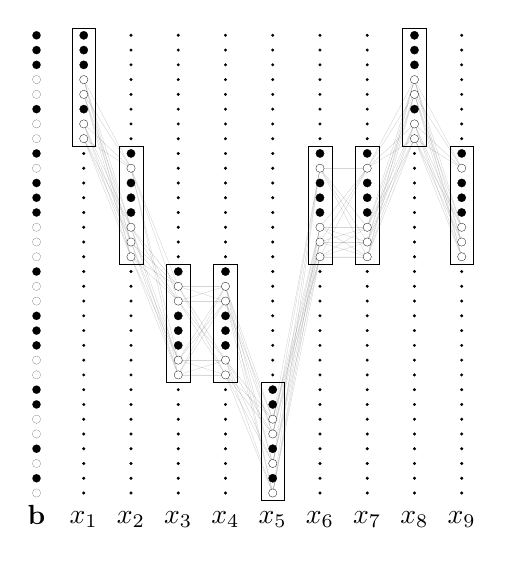
\begin{tikzpicture}%
\path[draw,line width=0.01pt,fill=white,radius=1.5pt] (0.0,0.0) circle;%
\path[draw,line width=0.01pt,fill=black,radius=1.5pt] (0.0,0.1875) circle;%
\path[draw,line width=0.01pt,fill=white,radius=1.5pt] (0.0,0.375) circle;%
\path[draw,line width=0.01pt,fill=black,radius=1.5pt] (0.0,0.5625) circle;%
\path[draw,line width=0.01pt,fill=white,radius=1.5pt] (0.0,0.75) circle;%
\path[draw,line width=0.01pt,fill=white,radius=1.5pt] (0.0,0.9375) circle;%
\path[draw,line width=0.01pt,fill=black,radius=1.5pt] (0.0,1.125) circle;%
\path[draw,line width=0.01pt,fill=black,radius=1.5pt] (0.0,1.3125) circle;%
\path[draw,line width=0.01pt,fill=white,radius=1.5pt] (0.0,1.5) circle;%
\path[draw,line width=0.01pt,fill=white,radius=1.5pt] (0.0,1.6875) circle;%
\path[draw,line width=0.01pt,fill=black,radius=1.5pt] (0.0,1.875) circle;%
\path[draw,line width=0.01pt,fill=black,radius=1.5pt] (0.0,2.0625) circle;%
\path[draw,line width=0.01pt,fill=black,radius=1.5pt] (0.0,2.25) circle;%
\path[draw,line width=0.01pt,fill=white,radius=1.5pt] (0.0,2.4375) circle;%
\path[draw,line width=0.01pt,fill=white,radius=1.5pt] (0.0,2.625) circle;%
\path[draw,line width=0.01pt,fill=black,radius=1.5pt] (0.0,2.8125) circle;%
\path[draw,line width=0.01pt,fill=white,radius=1.5pt] (0.0,3.0) circle;%
\path[draw,line width=0.01pt,fill=white,radius=1.5pt] (0.0,3.1875) circle;%
\path[draw,line width=0.01pt,fill=white,radius=1.5pt] (0.0,3.375) circle;%
\path[draw,line width=0.01pt,fill=black,radius=1.5pt] (0.0,3.5625) circle;%
\path[draw,line width=0.01pt,fill=black,radius=1.5pt] (0.0,3.75) circle;%
\path[draw,line width=0.01pt,fill=black,radius=1.5pt] (0.0,3.9375) circle;%
\path[draw,line width=0.01pt,fill=white,radius=1.5pt] (0.0,4.125) circle;%
\path[draw,line width=0.01pt,fill=black,radius=1.5pt] (0.0,4.3125) circle;%
\path[draw,line width=0.01pt,fill=white,radius=1.5pt] (0.0,4.5) circle;%
\path[draw,line width=0.01pt,fill=white,radius=1.5pt] (0.0,4.6875) circle;%
\path[draw,line width=0.01pt,fill=black,radius=1.5pt] (0.0,4.875) circle;%
\path[draw,line width=0.01pt,fill=white,radius=1.5pt] (0.0,5.0625) circle;%
\path[draw,line width=0.01pt,fill=white,radius=1.5pt] (0.0,5.25) circle;%
\path[draw,line width=0.01pt,fill=black,radius=1.5pt] (0.0,5.4375) circle;%
\path[draw,line width=0.01pt,fill=black,radius=1.5pt] (0.0,5.625) circle;%
\path[draw,line width=0.01pt,fill=black,radius=1.5pt] (0.0,5.8125) circle;%
\path[draw,line width=0.1pt,opacity=0.15,fill=black] (0.6,4.5) -- (1.2,3.0);%
\path[draw,line width=0.1pt,opacity=0.15,fill=black] (0.6,4.5) -- (1.2,3.1875);%
\path[draw,line width=0.1pt,opacity=0.15,fill=black] (0.6,4.5) -- (1.2,3.375);%
\path[draw,line width=0.1pt,opacity=0.15,fill=black] (0.6,4.5) -- (1.2,4.125);%
\path[draw,line width=0.1pt,opacity=0.15,fill=black] (0.6,4.6875) -- (1.2,3.0);%
\path[draw,line width=0.1pt,opacity=0.15,fill=black] (0.6,4.6875) -- (1.2,3.1875);%
\path[draw,line width=0.1pt,opacity=0.15,fill=black] (0.6,4.6875) -- (1.2,3.375);%
\path[draw,line width=0.1pt,opacity=0.15,fill=black] (0.6,4.6875) -- (1.2,4.125);%
\path[draw,line width=0.1pt,opacity=0.15,fill=black] (0.6,5.0625) -- (1.2,3.0);%
\path[draw,line width=0.1pt,opacity=0.15,fill=black] (0.6,5.0625) -- (1.2,3.1875);%
\path[draw,line width=0.1pt,opacity=0.15,fill=black] (0.6,5.0625) -- (1.2,3.375);%
\path[draw,line width=0.1pt,opacity=0.15,fill=black] (0.6,5.0625) -- (1.2,4.125);%
\path[draw,line width=0.1pt,opacity=0.15,fill=black] (0.6,5.25) -- (1.2,3.0);%
\path[draw,line width=0.1pt,opacity=0.15,fill=black] (0.6,5.25) -- (1.2,3.1875);%
\path[draw,line width=0.1pt,opacity=0.15,fill=black] (0.6,5.25) -- (1.2,3.375);%
\path[draw,line width=0.1pt,opacity=0.15,fill=black] (0.6,5.25) -- (1.2,4.125);%
\path[draw,line width=0.1pt,opacity=0.15,fill=black] (1.2,3.0) -- (1.8,1.5);%
\path[draw,line width=0.1pt,opacity=0.15,fill=black] (1.2,3.0) -- (1.8,1.6875);%
\path[draw,line width=0.1pt,opacity=0.15,fill=black] (1.2,3.0) -- (1.8,2.4375);%
\path[draw,line width=0.1pt,opacity=0.15,fill=black] (1.2,3.0) -- (1.8,2.625);%
\path[draw,line width=0.1pt,opacity=0.15,fill=black] (1.2,3.1875) -- (1.8,1.5);%
\path[draw,line width=0.1pt,opacity=0.15,fill=black] (1.2,3.1875) -- (1.8,1.6875);%
\path[draw,line width=0.1pt,opacity=0.15,fill=black] (1.2,3.1875) -- (1.8,2.4375);%
\path[draw,line width=0.1pt,opacity=0.15,fill=black] (1.2,3.1875) -- (1.8,2.625);%
\path[draw,line width=0.1pt,opacity=0.15,fill=black] (1.2,3.375) -- (1.8,1.5);%
\path[draw,line width=0.1pt,opacity=0.15,fill=black] (1.2,3.375) -- (1.8,1.6875);%
\path[draw,line width=0.1pt,opacity=0.15,fill=black] (1.2,3.375) -- (1.8,2.4375);%
\path[draw,line width=0.1pt,opacity=0.15,fill=black] (1.2,3.375) -- (1.8,2.625);%
\path[draw,line width=0.1pt,opacity=0.15,fill=black] (1.2,4.125) -- (1.8,1.5);%
\path[draw,line width=0.1pt,opacity=0.15,fill=black] (1.2,4.125) -- (1.8,1.6875);%
\path[draw,line width=0.1pt,opacity=0.15,fill=black] (1.2,4.125) -- (1.8,2.4375);%
\path[draw,line width=0.1pt,opacity=0.15,fill=black] (1.2,4.125) -- (1.8,2.625);%
\path[draw,line width=0.1pt,opacity=0.15,fill=black] (1.8,1.5) -- (2.4,1.5);%
\path[draw,line width=0.1pt,opacity=0.15,fill=black] (1.8,1.5) -- (2.4,1.6875);%
\path[draw,line width=0.1pt,opacity=0.15,fill=black] (1.8,1.5) -- (2.4,2.4375);%
\path[draw,line width=0.1pt,opacity=0.15,fill=black] (1.8,1.5) -- (2.4,2.625);%
\path[draw,line width=0.1pt,opacity=0.15,fill=black] (1.8,1.6875) -- (2.4,1.5);%
\path[draw,line width=0.1pt,opacity=0.15,fill=black] (1.8,1.6875) -- (2.4,1.6875);%
\path[draw,line width=0.1pt,opacity=0.15,fill=black] (1.8,1.6875) -- (2.4,2.4375);%
\path[draw,line width=0.1pt,opacity=0.15,fill=black] (1.8,1.6875) -- (2.4,2.625);%
\path[draw,line width=0.1pt,opacity=0.15,fill=black] (1.8,2.4375) -- (2.4,1.5);%
\path[draw,line width=0.1pt,opacity=0.15,fill=black] (1.8,2.4375) -- (2.4,1.6875);%
\path[draw,line width=0.1pt,opacity=0.15,fill=black] (1.8,2.4375) -- (2.4,2.4375);%
\path[draw,line width=0.1pt,opacity=0.15,fill=black] (1.8,2.4375) -- (2.4,2.625);%
\path[draw,line width=0.1pt,opacity=0.15,fill=black] (1.8,2.625) -- (2.4,1.5);%
\path[draw,line width=0.1pt,opacity=0.15,fill=black] (1.8,2.625) -- (2.4,1.6875);%
\path[draw,line width=0.1pt,opacity=0.15,fill=black] (1.8,2.625) -- (2.4,2.4375);%
\path[draw,line width=0.1pt,opacity=0.15,fill=black] (1.8,2.625) -- (2.4,2.625);%
\path[draw,line width=0.1pt,opacity=0.15,fill=black] (2.4,1.5) -- (3.0,0.0);%
\path[draw,line width=0.1pt,opacity=0.15,fill=black] (2.4,1.5) -- (3.0,0.375);%
\path[draw,line width=0.1pt,opacity=0.15,fill=black] (2.4,1.5) -- (3.0,0.75);%
\path[draw,line width=0.1pt,opacity=0.15,fill=black] (2.4,1.5) -- (3.0,0.9375);%
\path[draw,line width=0.1pt,opacity=0.15,fill=black] (2.4,1.6875) -- (3.0,0.0);%
\path[draw,line width=0.1pt,opacity=0.15,fill=black] (2.4,1.6875) -- (3.0,0.375);%
\path[draw,line width=0.1pt,opacity=0.15,fill=black] (2.4,1.6875) -- (3.0,0.75);%
\path[draw,line width=0.1pt,opacity=0.15,fill=black] (2.4,1.6875) -- (3.0,0.9375);%
\path[draw,line width=0.1pt,opacity=0.15,fill=black] (2.4,2.4375) -- (3.0,0.0);%
\path[draw,line width=0.1pt,opacity=0.15,fill=black] (2.4,2.4375) -- (3.0,0.375);%
\path[draw,line width=0.1pt,opacity=0.15,fill=black] (2.4,2.4375) -- (3.0,0.75);%
\path[draw,line width=0.1pt,opacity=0.15,fill=black] (2.4,2.4375) -- (3.0,0.9375);%
\path[draw,line width=0.1pt,opacity=0.15,fill=black] (2.4,2.625) -- (3.0,0.0);%
\path[draw,line width=0.1pt,opacity=0.15,fill=black] (2.4,2.625) -- (3.0,0.375);%
\path[draw,line width=0.1pt,opacity=0.15,fill=black] (2.4,2.625) -- (3.0,0.75);%
\path[draw,line width=0.1pt,opacity=0.15,fill=black] (2.4,2.625) -- (3.0,0.9375);%
\path[draw,line width=0.1pt,opacity=0.15,fill=black] (3.0,0.0) -- (3.6,3.0);%
\path[draw,line width=0.1pt,opacity=0.15,fill=black] (3.0,0.0) -- (3.6,3.1875);%
\path[draw,line width=0.1pt,opacity=0.15,fill=black] (3.0,0.0) -- (3.6,3.375);%
\path[draw,line width=0.1pt,opacity=0.15,fill=black] (3.0,0.0) -- (3.6,4.125);%
\path[draw,line width=0.1pt,opacity=0.15,fill=black] (3.0,0.375) -- (3.6,3.0);%
\path[draw,line width=0.1pt,opacity=0.15,fill=black] (3.0,0.375) -- (3.6,3.1875);%
\path[draw,line width=0.1pt,opacity=0.15,fill=black] (3.0,0.375) -- (3.6,3.375);%
\path[draw,line width=0.1pt,opacity=0.15,fill=black] (3.0,0.375) -- (3.6,4.125);%
\path[draw,line width=0.1pt,opacity=0.15,fill=black] (3.0,0.75) -- (3.6,3.0);%
\path[draw,line width=0.1pt,opacity=0.15,fill=black] (3.0,0.75) -- (3.6,3.1875);%
\path[draw,line width=0.1pt,opacity=0.15,fill=black] (3.0,0.75) -- (3.6,3.375);%
\path[draw,line width=0.1pt,opacity=0.15,fill=black] (3.0,0.75) -- (3.6,4.125);%
\path[draw,line width=0.1pt,opacity=0.15,fill=black] (3.0,0.9375) -- (3.6,3.0);%
\path[draw,line width=0.1pt,opacity=0.15,fill=black] (3.0,0.9375) -- (3.6,3.1875);%
\path[draw,line width=0.1pt,opacity=0.15,fill=black] (3.0,0.9375) -- (3.6,3.375);%
\path[draw,line width=0.1pt,opacity=0.15,fill=black] (3.0,0.9375) -- (3.6,4.125);%
\path[draw,line width=0.1pt,opacity=0.15,fill=black] (3.6,3.0) -- (4.2,3.0);%
\path[draw,line width=0.1pt,opacity=0.15,fill=black] (3.6,3.0) -- (4.2,3.1875);%
\path[draw,line width=0.1pt,opacity=0.15,fill=black] (3.6,3.0) -- (4.2,3.375);%
\path[draw,line width=0.1pt,opacity=0.15,fill=black] (3.6,3.0) -- (4.2,4.125);%
\path[draw,line width=0.1pt,opacity=0.15,fill=black] (3.6,3.1875) -- (4.2,3.0);%
\path[draw,line width=0.1pt,opacity=0.15,fill=black] (3.6,3.1875) -- (4.2,3.1875);%
\path[draw,line width=0.1pt,opacity=0.15,fill=black] (3.6,3.1875) -- (4.2,3.375);%
\path[draw,line width=0.1pt,opacity=0.15,fill=black] (3.6,3.1875) -- (4.2,4.125);%
\path[draw,line width=0.1pt,opacity=0.15,fill=black] (3.6,3.375) -- (4.2,3.0);%
\path[draw,line width=0.1pt,opacity=0.15,fill=black] (3.6,3.375) -- (4.2,3.1875);%
\path[draw,line width=0.1pt,opacity=0.15,fill=black] (3.6,3.375) -- (4.2,3.375);%
\path[draw,line width=0.1pt,opacity=0.15,fill=black] (3.6,3.375) -- (4.2,4.125);%
\path[draw,line width=0.1pt,opacity=0.15,fill=black] (3.6,4.125) -- (4.2,3.0);%
\path[draw,line width=0.1pt,opacity=0.15,fill=black] (3.6,4.125) -- (4.2,3.1875);%
\path[draw,line width=0.1pt,opacity=0.15,fill=black] (3.6,4.125) -- (4.2,3.375);%
\path[draw,line width=0.1pt,opacity=0.15,fill=black] (3.6,4.125) -- (4.2,4.125);%
\path[draw,line width=0.1pt,opacity=0.15,fill=black] (4.2,3.0) -- (4.8,4.5);%
\path[draw,line width=0.1pt,opacity=0.15,fill=black] (4.2,3.0) -- (4.8,4.6875);%
\path[draw,line width=0.1pt,opacity=0.15,fill=black] (4.2,3.0) -- (4.8,5.0625);%
\path[draw,line width=0.1pt,opacity=0.15,fill=black] (4.2,3.0) -- (4.8,5.25);%
\path[draw,line width=0.1pt,opacity=0.15,fill=black] (4.2,3.1875) -- (4.8,4.5);%
\path[draw,line width=0.1pt,opacity=0.15,fill=black] (4.2,3.1875) -- (4.8,4.6875);%
\path[draw,line width=0.1pt,opacity=0.15,fill=black] (4.2,3.1875) -- (4.8,5.0625);%
\path[draw,line width=0.1pt,opacity=0.15,fill=black] (4.2,3.1875) -- (4.8,5.25);%
\path[draw,line width=0.1pt,opacity=0.15,fill=black] (4.2,3.375) -- (4.8,4.5);%
\path[draw,line width=0.1pt,opacity=0.15,fill=black] (4.2,3.375) -- (4.8,4.6875);%
\path[draw,line width=0.1pt,opacity=0.15,fill=black] (4.2,3.375) -- (4.8,5.0625);%
\path[draw,line width=0.1pt,opacity=0.15,fill=black] (4.2,3.375) -- (4.8,5.25);%
\path[draw,line width=0.1pt,opacity=0.15,fill=black] (4.2,4.125) -- (4.8,4.5);%
\path[draw,line width=0.1pt,opacity=0.15,fill=black] (4.2,4.125) -- (4.8,4.6875);%
\path[draw,line width=0.1pt,opacity=0.15,fill=black] (4.2,4.125) -- (4.8,5.0625);%
\path[draw,line width=0.1pt,opacity=0.15,fill=black] (4.2,4.125) -- (4.8,5.25);%
\path[draw,line width=0.1pt,opacity=0.15,fill=black] (4.8,4.5) -- (5.4,3.0);%
\path[draw,line width=0.1pt,opacity=0.15,fill=black] (4.8,4.5) -- (5.4,3.1875);%
\path[draw,line width=0.1pt,opacity=0.15,fill=black] (4.8,4.5) -- (5.4,3.375);%
\path[draw,line width=0.1pt,opacity=0.15,fill=black] (4.8,4.5) -- (5.4,4.125);%
\path[draw,line width=0.1pt,opacity=0.15,fill=black] (4.8,4.6875) -- (5.4,3.0);%
\path[draw,line width=0.1pt,opacity=0.15,fill=black] (4.8,4.6875) -- (5.4,3.1875);%
\path[draw,line width=0.1pt,opacity=0.15,fill=black] (4.8,4.6875) -- (5.4,3.375);%
\path[draw,line width=0.1pt,opacity=0.15,fill=black] (4.8,4.6875) -- (5.4,4.125);%
\path[draw,line width=0.1pt,opacity=0.15,fill=black] (4.8,5.0625) -- (5.4,3.0);%
\path[draw,line width=0.1pt,opacity=0.15,fill=black] (4.8,5.0625) -- (5.4,3.1875);%
\path[draw,line width=0.1pt,opacity=0.15,fill=black] (4.8,5.0625) -- (5.4,3.375);%
\path[draw,line width=0.1pt,opacity=0.15,fill=black] (4.8,5.0625) -- (5.4,4.125);%
\path[draw,line width=0.1pt,opacity=0.15,fill=black] (4.8,5.25) -- (5.4,3.0);%
\path[draw,line width=0.1pt,opacity=0.15,fill=black] (4.8,5.25) -- (5.4,3.1875);%
\path[draw,line width=0.1pt,opacity=0.15,fill=black] (4.8,5.25) -- (5.4,3.375);%
\path[draw,line width=0.1pt,opacity=0.15,fill=black] (4.8,5.25) -- (5.4,4.125);%
\path[draw,line width=0.2pt] (0.45,4.40625) rectangle (0.75,5.90625);%
\path[draw,line width=0.2pt] (1.05,2.90625) rectangle (1.35,4.40625);%
\path[draw,line width=0.2pt] (1.65,1.40625) rectangle (1.95,2.90625);%
\path[draw,line width=0.2pt] (2.25,1.40625) rectangle (2.55,2.90625);%
\path[draw,line width=0.2pt] (2.85,-0.09375) rectangle (3.15,1.40625);%
\path[draw,line width=0.2pt] (3.45,2.90625) rectangle (3.75,4.40625);%
\path[draw,line width=0.2pt] (4.05,2.90625) rectangle (4.35,4.40625);%
\path[draw,line width=0.2pt] (4.65,4.40625) rectangle (4.95,5.90625);%
\path[draw,line width=0.2pt] (5.25,2.90625) rectangle (5.55,4.40625);%
\node[inner sep=0] (b) at (0.0,-0.28125) {$\mathbf{b}$};%
\node (x1) at (0.6,-0.3375) {$x_1$};%
\node (x2) at (1.2,-0.3375) {$x_2$};%
\node (x3) at (1.8,-0.3375) {$x_3$};%
\node (x4) at (2.4,-0.3375) {$x_4$};%
\node (x5) at (3.0,-0.3375) {$x_5$};%
\node (x6) at (3.6,-0.3375) {$x_6$};%
\node (x7) at (4.2,-0.3375) {$x_7$};%
\node (x8) at (4.8,-0.3375) {$x_8$};%
\node (x9) at (5.4,-0.3375) {$x_9$};%
\path[draw,line width=0.1pt,fill=black,radius=0.5pt] (0.6,0.0) circle;%
\path[draw,line width=0.1pt,fill=black,radius=0.5pt] (0.6,0.1875) circle;%
\path[draw,line width=0.1pt,fill=black,radius=0.5pt] (0.6,0.375) circle;%
\path[draw,line width=0.1pt,fill=black,radius=0.5pt] (0.6,0.5625) circle;%
\path[draw,line width=0.1pt,fill=black,radius=0.5pt] (0.6,0.75) circle;%
\path[draw,line width=0.1pt,fill=black,radius=0.5pt] (0.6,0.9375) circle;%
\path[draw,line width=0.1pt,fill=black,radius=0.5pt] (0.6,1.125) circle;%
\path[draw,line width=0.1pt,fill=black,radius=0.5pt] (0.6,1.3125) circle;%
\path[draw,line width=0.1pt,fill=black,radius=0.5pt] (0.6,1.5) circle;%
\path[draw,line width=0.1pt,fill=black,radius=0.5pt] (0.6,1.6875) circle;%
\path[draw,line width=0.1pt,fill=black,radius=0.5pt] (0.6,1.875) circle;%
\path[draw,line width=0.1pt,fill=black,radius=0.5pt] (0.6,2.0625) circle;%
\path[draw,line width=0.1pt,fill=black,radius=0.5pt] (0.6,2.25) circle;%
\path[draw,line width=0.1pt,fill=black,radius=0.5pt] (0.6,2.4375) circle;%
\path[draw,line width=0.1pt,fill=black,radius=0.5pt] (0.6,2.625) circle;%
\path[draw,line width=0.1pt,fill=black,radius=0.5pt] (0.6,2.8125) circle;%
\path[draw,line width=0.1pt,fill=black,radius=0.5pt] (0.6,3.0) circle;%
\path[draw,line width=0.1pt,fill=black,radius=0.5pt] (0.6,3.1875) circle;%
\path[draw,line width=0.1pt,fill=black,radius=0.5pt] (0.6,3.375) circle;%
\path[draw,line width=0.1pt,fill=black,radius=0.5pt] (0.6,3.5625) circle;%
\path[draw,line width=0.1pt,fill=black,radius=0.5pt] (0.6,3.75) circle;%
\path[draw,line width=0.1pt,fill=black,radius=0.5pt] (0.6,3.9375) circle;%
\path[draw,line width=0.1pt,fill=black,radius=0.5pt] (0.6,4.125) circle;%
\path[draw,line width=0.1pt,fill=black,radius=0.5pt] (0.6,4.3125) circle;%
\path[draw,line width=0.1pt,fill=white,radius=1.5pt] (0.6,4.5) circle;%
\path[draw,line width=0.1pt,fill=white,radius=1.5pt] (0.6,4.6875) circle;%
\path[draw,line width=0.1pt,fill=black,radius=1.5pt] (0.6,4.875) circle;%
\path[draw,line width=0.1pt,fill=white,radius=1.5pt] (0.6,5.0625) circle;%
\path[draw,line width=0.1pt,fill=white,radius=1.5pt] (0.6,5.25) circle;%
\path[draw,line width=0.1pt,fill=black,radius=1.5pt] (0.6,5.4375) circle;%
\path[draw,line width=0.1pt,fill=black,radius=1.5pt] (0.6,5.625) circle;%
\path[draw,line width=0.1pt,fill=black,radius=1.5pt] (0.6,5.8125) circle;%
\path[draw,line width=0.1pt,fill=black,radius=0.5pt] (1.2,0.0) circle;%
\path[draw,line width=0.1pt,fill=black,radius=0.5pt] (1.2,0.1875) circle;%
\path[draw,line width=0.1pt,fill=black,radius=0.5pt] (1.2,0.375) circle;%
\path[draw,line width=0.1pt,fill=black,radius=0.5pt] (1.2,0.5625) circle;%
\path[draw,line width=0.1pt,fill=black,radius=0.5pt] (1.2,0.75) circle;%
\path[draw,line width=0.1pt,fill=black,radius=0.5pt] (1.2,0.9375) circle;%
\path[draw,line width=0.1pt,fill=black,radius=0.5pt] (1.2,1.125) circle;%
\path[draw,line width=0.1pt,fill=black,radius=0.5pt] (1.2,1.3125) circle;%
\path[draw,line width=0.1pt,fill=black,radius=0.5pt] (1.2,1.5) circle;%
\path[draw,line width=0.1pt,fill=black,radius=0.5pt] (1.2,1.6875) circle;%
\path[draw,line width=0.1pt,fill=black,radius=0.5pt] (1.2,1.875) circle;%
\path[draw,line width=0.1pt,fill=black,radius=0.5pt] (1.2,2.0625) circle;%
\path[draw,line width=0.1pt,fill=black,radius=0.5pt] (1.2,2.25) circle;%
\path[draw,line width=0.1pt,fill=black,radius=0.5pt] (1.2,2.4375) circle;%
\path[draw,line width=0.1pt,fill=black,radius=0.5pt] (1.2,2.625) circle;%
\path[draw,line width=0.1pt,fill=black,radius=0.5pt] (1.2,2.8125) circle;%
\path[draw,line width=0.1pt,fill=white,radius=1.5pt] (1.2,3.0) circle;%
\path[draw,line width=0.1pt,fill=white,radius=1.5pt] (1.2,3.1875) circle;%
\path[draw,line width=0.1pt,fill=white,radius=1.5pt] (1.2,3.375) circle;%
\path[draw,line width=0.1pt,fill=black,radius=1.5pt] (1.2,3.5625) circle;%
\path[draw,line width=0.1pt,fill=black,radius=1.5pt] (1.2,3.75) circle;%
\path[draw,line width=0.1pt,fill=black,radius=1.5pt] (1.2,3.9375) circle;%
\path[draw,line width=0.1pt,fill=white,radius=1.5pt] (1.2,4.125) circle;%
\path[draw,line width=0.1pt,fill=black,radius=1.5pt] (1.2,4.3125) circle;%
\path[draw,line width=0.1pt,fill=black,radius=0.5pt] (1.2,4.5) circle;%
\path[draw,line width=0.1pt,fill=black,radius=0.5pt] (1.2,4.6875) circle;%
\path[draw,line width=0.1pt,fill=black,radius=0.5pt] (1.2,4.875) circle;%
\path[draw,line width=0.1pt,fill=black,radius=0.5pt] (1.2,5.0625) circle;%
\path[draw,line width=0.1pt,fill=black,radius=0.5pt] (1.2,5.25) circle;%
\path[draw,line width=0.1pt,fill=black,radius=0.5pt] (1.2,5.4375) circle;%
\path[draw,line width=0.1pt,fill=black,radius=0.5pt] (1.2,5.625) circle;%
\path[draw,line width=0.1pt,fill=black,radius=0.5pt] (1.2,5.8125) circle;%
\path[draw,line width=0.1pt,fill=black,radius=0.5pt] (1.8,0.0) circle;%
\path[draw,line width=0.1pt,fill=black,radius=0.5pt] (1.8,0.1875) circle;%
\path[draw,line width=0.1pt,fill=black,radius=0.5pt] (1.8,0.375) circle;%
\path[draw,line width=0.1pt,fill=black,radius=0.5pt] (1.8,0.5625) circle;%
\path[draw,line width=0.1pt,fill=black,radius=0.5pt] (1.8,0.75) circle;%
\path[draw,line width=0.1pt,fill=black,radius=0.5pt] (1.8,0.9375) circle;%
\path[draw,line width=0.1pt,fill=black,radius=0.5pt] (1.8,1.125) circle;%
\path[draw,line width=0.1pt,fill=black,radius=0.5pt] (1.8,1.3125) circle;%
\path[draw,line width=0.1pt,fill=white,radius=1.5pt] (1.8,1.5) circle;%
\path[draw,line width=0.1pt,fill=white,radius=1.5pt] (1.8,1.6875) circle;%
\path[draw,line width=0.1pt,fill=black,radius=1.5pt] (1.8,1.875) circle;%
\path[draw,line width=0.1pt,fill=black,radius=1.5pt] (1.8,2.0625) circle;%
\path[draw,line width=0.1pt,fill=black,radius=1.5pt] (1.8,2.25) circle;%
\path[draw,line width=0.1pt,fill=white,radius=1.5pt] (1.8,2.4375) circle;%
\path[draw,line width=0.1pt,fill=white,radius=1.5pt] (1.8,2.625) circle;%
\path[draw,line width=0.1pt,fill=black,radius=1.5pt] (1.8,2.8125) circle;%
\path[draw,line width=0.1pt,fill=black,radius=0.5pt] (1.8,3.0) circle;%
\path[draw,line width=0.1pt,fill=black,radius=0.5pt] (1.8,3.1875) circle;%
\path[draw,line width=0.1pt,fill=black,radius=0.5pt] (1.8,3.375) circle;%
\path[draw,line width=0.1pt,fill=black,radius=0.5pt] (1.8,3.5625) circle;%
\path[draw,line width=0.1pt,fill=black,radius=0.5pt] (1.8,3.75) circle;%
\path[draw,line width=0.1pt,fill=black,radius=0.5pt] (1.8,3.9375) circle;%
\path[draw,line width=0.1pt,fill=black,radius=0.5pt] (1.8,4.125) circle;%
\path[draw,line width=0.1pt,fill=black,radius=0.5pt] (1.8,4.3125) circle;%
\path[draw,line width=0.1pt,fill=black,radius=0.5pt] (1.8,4.5) circle;%
\path[draw,line width=0.1pt,fill=black,radius=0.5pt] (1.8,4.6875) circle;%
\path[draw,line width=0.1pt,fill=black,radius=0.5pt] (1.8,4.875) circle;%
\path[draw,line width=0.1pt,fill=black,radius=0.5pt] (1.8,5.0625) circle;%
\path[draw,line width=0.1pt,fill=black,radius=0.5pt] (1.8,5.25) circle;%
\path[draw,line width=0.1pt,fill=black,radius=0.5pt] (1.8,5.4375) circle;%
\path[draw,line width=0.1pt,fill=black,radius=0.5pt] (1.8,5.625) circle;%
\path[draw,line width=0.1pt,fill=black,radius=0.5pt] (1.8,5.8125) circle;%
\path[draw,line width=0.1pt,fill=black,radius=0.5pt] (2.4,0.0) circle;%
\path[draw,line width=0.1pt,fill=black,radius=0.5pt] (2.4,0.1875) circle;%
\path[draw,line width=0.1pt,fill=black,radius=0.5pt] (2.4,0.375) circle;%
\path[draw,line width=0.1pt,fill=black,radius=0.5pt] (2.4,0.5625) circle;%
\path[draw,line width=0.1pt,fill=black,radius=0.5pt] (2.4,0.75) circle;%
\path[draw,line width=0.1pt,fill=black,radius=0.5pt] (2.4,0.9375) circle;%
\path[draw,line width=0.1pt,fill=black,radius=0.5pt] (2.4,1.125) circle;%
\path[draw,line width=0.1pt,fill=black,radius=0.5pt] (2.4,1.3125) circle;%
\path[draw,line width=0.1pt,fill=white,radius=1.5pt] (2.4,1.5) circle;%
\path[draw,line width=0.1pt,fill=white,radius=1.5pt] (2.4,1.6875) circle;%
\path[draw,line width=0.1pt,fill=black,radius=1.5pt] (2.4,1.875) circle;%
\path[draw,line width=0.1pt,fill=black,radius=1.5pt] (2.4,2.0625) circle;%
\path[draw,line width=0.1pt,fill=black,radius=1.5pt] (2.4,2.25) circle;%
\path[draw,line width=0.1pt,fill=white,radius=1.5pt] (2.4,2.4375) circle;%
\path[draw,line width=0.1pt,fill=white,radius=1.5pt] (2.4,2.625) circle;%
\path[draw,line width=0.1pt,fill=black,radius=1.5pt] (2.4,2.8125) circle;%
\path[draw,line width=0.1pt,fill=black,radius=0.5pt] (2.4,3.0) circle;%
\path[draw,line width=0.1pt,fill=black,radius=0.5pt] (2.4,3.1875) circle;%
\path[draw,line width=0.1pt,fill=black,radius=0.5pt] (2.4,3.375) circle;%
\path[draw,line width=0.1pt,fill=black,radius=0.5pt] (2.4,3.5625) circle;%
\path[draw,line width=0.1pt,fill=black,radius=0.5pt] (2.4,3.75) circle;%
\path[draw,line width=0.1pt,fill=black,radius=0.5pt] (2.4,3.9375) circle;%
\path[draw,line width=0.1pt,fill=black,radius=0.5pt] (2.4,4.125) circle;%
\path[draw,line width=0.1pt,fill=black,radius=0.5pt] (2.4,4.3125) circle;%
\path[draw,line width=0.1pt,fill=black,radius=0.5pt] (2.4,4.5) circle;%
\path[draw,line width=0.1pt,fill=black,radius=0.5pt] (2.4,4.6875) circle;%
\path[draw,line width=0.1pt,fill=black,radius=0.5pt] (2.4,4.875) circle;%
\path[draw,line width=0.1pt,fill=black,radius=0.5pt] (2.4,5.0625) circle;%
\path[draw,line width=0.1pt,fill=black,radius=0.5pt] (2.4,5.25) circle;%
\path[draw,line width=0.1pt,fill=black,radius=0.5pt] (2.4,5.4375) circle;%
\path[draw,line width=0.1pt,fill=black,radius=0.5pt] (2.4,5.625) circle;%
\path[draw,line width=0.1pt,fill=black,radius=0.5pt] (2.4,5.8125) circle;%
\path[draw,line width=0.1pt,fill=white,radius=1.5pt] (3.0,0.0) circle;%
\path[draw,line width=0.1pt,fill=black,radius=1.5pt] (3.0,0.1875) circle;%
\path[draw,line width=0.1pt,fill=white,radius=1.5pt] (3.0,0.375) circle;%
\path[draw,line width=0.1pt,fill=black,radius=1.5pt] (3.0,0.5625) circle;%
\path[draw,line width=0.1pt,fill=white,radius=1.5pt] (3.0,0.75) circle;%
\path[draw,line width=0.1pt,fill=white,radius=1.5pt] (3.0,0.9375) circle;%
\path[draw,line width=0.1pt,fill=black,radius=1.5pt] (3.0,1.125) circle;%
\path[draw,line width=0.1pt,fill=black,radius=1.5pt] (3.0,1.3125) circle;%
\path[draw,line width=0.1pt,fill=black,radius=0.5pt] (3.0,1.5) circle;%
\path[draw,line width=0.1pt,fill=black,radius=0.5pt] (3.0,1.6875) circle;%
\path[draw,line width=0.1pt,fill=black,radius=0.5pt] (3.0,1.875) circle;%
\path[draw,line width=0.1pt,fill=black,radius=0.5pt] (3.0,2.0625) circle;%
\path[draw,line width=0.1pt,fill=black,radius=0.5pt] (3.0,2.25) circle;%
\path[draw,line width=0.1pt,fill=black,radius=0.5pt] (3.0,2.4375) circle;%
\path[draw,line width=0.1pt,fill=black,radius=0.5pt] (3.0,2.625) circle;%
\path[draw,line width=0.1pt,fill=black,radius=0.5pt] (3.0,2.8125) circle;%
\path[draw,line width=0.1pt,fill=black,radius=0.5pt] (3.0,3.0) circle;%
\path[draw,line width=0.1pt,fill=black,radius=0.5pt] (3.0,3.1875) circle;%
\path[draw,line width=0.1pt,fill=black,radius=0.5pt] (3.0,3.375) circle;%
\path[draw,line width=0.1pt,fill=black,radius=0.5pt] (3.0,3.5625) circle;%
\path[draw,line width=0.1pt,fill=black,radius=0.5pt] (3.0,3.75) circle;%
\path[draw,line width=0.1pt,fill=black,radius=0.5pt] (3.0,3.9375) circle;%
\path[draw,line width=0.1pt,fill=black,radius=0.5pt] (3.0,4.125) circle;%
\path[draw,line width=0.1pt,fill=black,radius=0.5pt] (3.0,4.3125) circle;%
\path[draw,line width=0.1pt,fill=black,radius=0.5pt] (3.0,4.5) circle;%
\path[draw,line width=0.1pt,fill=black,radius=0.5pt] (3.0,4.6875) circle;%
\path[draw,line width=0.1pt,fill=black,radius=0.5pt] (3.0,4.875) circle;%
\path[draw,line width=0.1pt,fill=black,radius=0.5pt] (3.0,5.0625) circle;%
\path[draw,line width=0.1pt,fill=black,radius=0.5pt] (3.0,5.25) circle;%
\path[draw,line width=0.1pt,fill=black,radius=0.5pt] (3.0,5.4375) circle;%
\path[draw,line width=0.1pt,fill=black,radius=0.5pt] (3.0,5.625) circle;%
\path[draw,line width=0.1pt,fill=black,radius=0.5pt] (3.0,5.8125) circle;%
\path[draw,line width=0.1pt,fill=black,radius=0.5pt] (3.6,0.0) circle;%
\path[draw,line width=0.1pt,fill=black,radius=0.5pt] (3.6,0.1875) circle;%
\path[draw,line width=0.1pt,fill=black,radius=0.5pt] (3.6,0.375) circle;%
\path[draw,line width=0.1pt,fill=black,radius=0.5pt] (3.6,0.5625) circle;%
\path[draw,line width=0.1pt,fill=black,radius=0.5pt] (3.6,0.75) circle;%
\path[draw,line width=0.1pt,fill=black,radius=0.5pt] (3.6,0.9375) circle;%
\path[draw,line width=0.1pt,fill=black,radius=0.5pt] (3.6,1.125) circle;%
\path[draw,line width=0.1pt,fill=black,radius=0.5pt] (3.6,1.3125) circle;%
\path[draw,line width=0.1pt,fill=black,radius=0.5pt] (3.6,1.5) circle;%
\path[draw,line width=0.1pt,fill=black,radius=0.5pt] (3.6,1.6875) circle;%
\path[draw,line width=0.1pt,fill=black,radius=0.5pt] (3.6,1.875) circle;%
\path[draw,line width=0.1pt,fill=black,radius=0.5pt] (3.6,2.0625) circle;%
\path[draw,line width=0.1pt,fill=black,radius=0.5pt] (3.6,2.25) circle;%
\path[draw,line width=0.1pt,fill=black,radius=0.5pt] (3.6,2.4375) circle;%
\path[draw,line width=0.1pt,fill=black,radius=0.5pt] (3.6,2.625) circle;%
\path[draw,line width=0.1pt,fill=black,radius=0.5pt] (3.6,2.8125) circle;%
\path[draw,line width=0.1pt,fill=white,radius=1.5pt] (3.6,3.0) circle;%
\path[draw,line width=0.1pt,fill=white,radius=1.5pt] (3.6,3.1875) circle;%
\path[draw,line width=0.1pt,fill=white,radius=1.5pt] (3.6,3.375) circle;%
\path[draw,line width=0.1pt,fill=black,radius=1.5pt] (3.6,3.5625) circle;%
\path[draw,line width=0.1pt,fill=black,radius=1.5pt] (3.6,3.75) circle;%
\path[draw,line width=0.1pt,fill=black,radius=1.5pt] (3.6,3.9375) circle;%
\path[draw,line width=0.1pt,fill=white,radius=1.5pt] (3.6,4.125) circle;%
\path[draw,line width=0.1pt,fill=black,radius=1.5pt] (3.6,4.3125) circle;%
\path[draw,line width=0.1pt,fill=black,radius=0.5pt] (3.6,4.5) circle;%
\path[draw,line width=0.1pt,fill=black,radius=0.5pt] (3.6,4.6875) circle;%
\path[draw,line width=0.1pt,fill=black,radius=0.5pt] (3.6,4.875) circle;%
\path[draw,line width=0.1pt,fill=black,radius=0.5pt] (3.6,5.0625) circle;%
\path[draw,line width=0.1pt,fill=black,radius=0.5pt] (3.6,5.25) circle;%
\path[draw,line width=0.1pt,fill=black,radius=0.5pt] (3.6,5.4375) circle;%
\path[draw,line width=0.1pt,fill=black,radius=0.5pt] (3.6,5.625) circle;%
\path[draw,line width=0.1pt,fill=black,radius=0.5pt] (3.6,5.8125) circle;%
\path[draw,line width=0.1pt,fill=black,radius=0.5pt] (4.2,0.0) circle;%
\path[draw,line width=0.1pt,fill=black,radius=0.5pt] (4.2,0.1875) circle;%
\path[draw,line width=0.1pt,fill=black,radius=0.5pt] (4.2,0.375) circle;%
\path[draw,line width=0.1pt,fill=black,radius=0.5pt] (4.2,0.5625) circle;%
\path[draw,line width=0.1pt,fill=black,radius=0.5pt] (4.2,0.75) circle;%
\path[draw,line width=0.1pt,fill=black,radius=0.5pt] (4.2,0.9375) circle;%
\path[draw,line width=0.1pt,fill=black,radius=0.5pt] (4.2,1.125) circle;%
\path[draw,line width=0.1pt,fill=black,radius=0.5pt] (4.2,1.3125) circle;%
\path[draw,line width=0.1pt,fill=black,radius=0.5pt] (4.2,1.5) circle;%
\path[draw,line width=0.1pt,fill=black,radius=0.5pt] (4.2,1.6875) circle;%
\path[draw,line width=0.1pt,fill=black,radius=0.5pt] (4.2,1.875) circle;%
\path[draw,line width=0.1pt,fill=black,radius=0.5pt] (4.2,2.0625) circle;%
\path[draw,line width=0.1pt,fill=black,radius=0.5pt] (4.2,2.25) circle;%
\path[draw,line width=0.1pt,fill=black,radius=0.5pt] (4.2,2.4375) circle;%
\path[draw,line width=0.1pt,fill=black,radius=0.5pt] (4.2,2.625) circle;%
\path[draw,line width=0.1pt,fill=black,radius=0.5pt] (4.2,2.8125) circle;%
\path[draw,line width=0.1pt,fill=white,radius=1.5pt] (4.2,3.0) circle;%
\path[draw,line width=0.1pt,fill=white,radius=1.5pt] (4.2,3.1875) circle;%
\path[draw,line width=0.1pt,fill=white,radius=1.5pt] (4.2,3.375) circle;%
\path[draw,line width=0.1pt,fill=black,radius=1.5pt] (4.2,3.5625) circle;%
\path[draw,line width=0.1pt,fill=black,radius=1.5pt] (4.2,3.75) circle;%
\path[draw,line width=0.1pt,fill=black,radius=1.5pt] (4.2,3.9375) circle;%
\path[draw,line width=0.1pt,fill=white,radius=1.5pt] (4.2,4.125) circle;%
\path[draw,line width=0.1pt,fill=black,radius=1.5pt] (4.2,4.3125) circle;%
\path[draw,line width=0.1pt,fill=black,radius=0.5pt] (4.2,4.5) circle;%
\path[draw,line width=0.1pt,fill=black,radius=0.5pt] (4.2,4.6875) circle;%
\path[draw,line width=0.1pt,fill=black,radius=0.5pt] (4.2,4.875) circle;%
\path[draw,line width=0.1pt,fill=black,radius=0.5pt] (4.2,5.0625) circle;%
\path[draw,line width=0.1pt,fill=black,radius=0.5pt] (4.2,5.25) circle;%
\path[draw,line width=0.1pt,fill=black,radius=0.5pt] (4.2,5.4375) circle;%
\path[draw,line width=0.1pt,fill=black,radius=0.5pt] (4.2,5.625) circle;%
\path[draw,line width=0.1pt,fill=black,radius=0.5pt] (4.2,5.8125) circle;%
\path[draw,line width=0.1pt,fill=black,radius=0.5pt] (4.8,0.0) circle;%
\path[draw,line width=0.1pt,fill=black,radius=0.5pt] (4.8,0.1875) circle;%
\path[draw,line width=0.1pt,fill=black,radius=0.5pt] (4.8,0.375) circle;%
\path[draw,line width=0.1pt,fill=black,radius=0.5pt] (4.8,0.5625) circle;%
\path[draw,line width=0.1pt,fill=black,radius=0.5pt] (4.8,0.75) circle;%
\path[draw,line width=0.1pt,fill=black,radius=0.5pt] (4.8,0.9375) circle;%
\path[draw,line width=0.1pt,fill=black,radius=0.5pt] (4.8,1.125) circle;%
\path[draw,line width=0.1pt,fill=black,radius=0.5pt] (4.8,1.3125) circle;%
\path[draw,line width=0.1pt,fill=black,radius=0.5pt] (4.8,1.5) circle;%
\path[draw,line width=0.1pt,fill=black,radius=0.5pt] (4.8,1.6875) circle;%
\path[draw,line width=0.1pt,fill=black,radius=0.5pt] (4.8,1.875) circle;%
\path[draw,line width=0.1pt,fill=black,radius=0.5pt] (4.8,2.0625) circle;%
\path[draw,line width=0.1pt,fill=black,radius=0.5pt] (4.8,2.25) circle;%
\path[draw,line width=0.1pt,fill=black,radius=0.5pt] (4.8,2.4375) circle;%
\path[draw,line width=0.1pt,fill=black,radius=0.5pt] (4.8,2.625) circle;%
\path[draw,line width=0.1pt,fill=black,radius=0.5pt] (4.8,2.8125) circle;%
\path[draw,line width=0.1pt,fill=black,radius=0.5pt] (4.8,3.0) circle;%
\path[draw,line width=0.1pt,fill=black,radius=0.5pt] (4.8,3.1875) circle;%
\path[draw,line width=0.1pt,fill=black,radius=0.5pt] (4.8,3.375) circle;%
\path[draw,line width=0.1pt,fill=black,radius=0.5pt] (4.8,3.5625) circle;%
\path[draw,line width=0.1pt,fill=black,radius=0.5pt] (4.8,3.75) circle;%
\path[draw,line width=0.1pt,fill=black,radius=0.5pt] (4.8,3.9375) circle;%
\path[draw,line width=0.1pt,fill=black,radius=0.5pt] (4.8,4.125) circle;%
\path[draw,line width=0.1pt,fill=black,radius=0.5pt] (4.8,4.3125) circle;%
\path[draw,line width=0.1pt,fill=white,radius=1.5pt] (4.8,4.5) circle;%
\path[draw,line width=0.1pt,fill=white,radius=1.5pt] (4.8,4.6875) circle;%
\path[draw,line width=0.1pt,fill=black,radius=1.5pt] (4.8,4.875) circle;%
\path[draw,line width=0.1pt,fill=white,radius=1.5pt] (4.8,5.0625) circle;%
\path[draw,line width=0.1pt,fill=white,radius=1.5pt] (4.8,5.25) circle;%
\path[draw,line width=0.1pt,fill=black,radius=1.5pt] (4.8,5.4375) circle;%
\path[draw,line width=0.1pt,fill=black,radius=1.5pt] (4.8,5.625) circle;%
\path[draw,line width=0.1pt,fill=black,radius=1.5pt] (4.8,5.8125) circle;%
\path[draw,line width=0.1pt,fill=black,radius=0.5pt] (5.4,0.0) circle;%
\path[draw,line width=0.1pt,fill=black,radius=0.5pt] (5.4,0.1875) circle;%
\path[draw,line width=0.1pt,fill=black,radius=0.5pt] (5.4,0.375) circle;%
\path[draw,line width=0.1pt,fill=black,radius=0.5pt] (5.4,0.5625) circle;%
\path[draw,line width=0.1pt,fill=black,radius=0.5pt] (5.4,0.75) circle;%
\path[draw,line width=0.1pt,fill=black,radius=0.5pt] (5.4,0.9375) circle;%
\path[draw,line width=0.1pt,fill=black,radius=0.5pt] (5.4,1.125) circle;%
\path[draw,line width=0.1pt,fill=black,radius=0.5pt] (5.4,1.3125) circle;%
\path[draw,line width=0.1pt,fill=black,radius=0.5pt] (5.4,1.5) circle;%
\path[draw,line width=0.1pt,fill=black,radius=0.5pt] (5.4,1.6875) circle;%
\path[draw,line width=0.1pt,fill=black,radius=0.5pt] (5.4,1.875) circle;%
\path[draw,line width=0.1pt,fill=black,radius=0.5pt] (5.4,2.0625) circle;%
\path[draw,line width=0.1pt,fill=black,radius=0.5pt] (5.4,2.25) circle;%
\path[draw,line width=0.1pt,fill=black,radius=0.5pt] (5.4,2.4375) circle;%
\path[draw,line width=0.1pt,fill=black,radius=0.5pt] (5.4,2.625) circle;%
\path[draw,line width=0.1pt,fill=black,radius=0.5pt] (5.4,2.8125) circle;%
\path[draw,line width=0.1pt,fill=white,radius=1.5pt] (5.4,3.0) circle;%
\path[draw,line width=0.1pt,fill=white,radius=1.5pt] (5.4,3.1875) circle;%
\path[draw,line width=0.1pt,fill=white,radius=1.5pt] (5.4,3.375) circle;%
\path[draw,line width=0.1pt,fill=black,radius=1.5pt] (5.4,3.5625) circle;%
\path[draw,line width=0.1pt,fill=black,radius=1.5pt] (5.4,3.75) circle;%
\path[draw,line width=0.1pt,fill=black,radius=1.5pt] (5.4,3.9375) circle;%
\path[draw,line width=0.1pt,fill=white,radius=1.5pt] (5.4,4.125) circle;%
\path[draw,line width=0.1pt,fill=black,radius=1.5pt] (5.4,4.3125) circle;%
\path[draw,line width=0.1pt,fill=black,radius=0.5pt] (5.4,4.5) circle;%
\path[draw,line width=0.1pt,fill=black,radius=0.5pt] (5.4,4.6875) circle;%
\path[draw,line width=0.1pt,fill=black,radius=0.5pt] (5.4,4.875) circle;%
\path[draw,line width=0.1pt,fill=black,radius=0.5pt] (5.4,5.0625) circle;%
\path[draw,line width=0.1pt,fill=black,radius=0.5pt] (5.4,5.25) circle;%
\path[draw,line width=0.1pt,fill=black,radius=0.5pt] (5.4,5.4375) circle;%
\path[draw,line width=0.1pt,fill=black,radius=0.5pt] (5.4,5.625) circle;%
\path[draw,line width=0.1pt,fill=black,radius=0.5pt] (5.4,5.8125) circle;%
\end{tikzpicture}%

\end{center}
\caption{
\label{fig:trellis}
The computation of $p(\bx)$ is greatly reduced by blocked emissions and state dropout.
In the above trellis, each row corresponds to a latent state.
Blocked emissions result in a small subset of all states emitting a given word,
as shown by the rectangles, thus only states in the rectangles may occur
with nonzero probability after conditioning on observed words.
State dropout (leftmost column) allows us to further reduce the number of states we consider,
halving the number of (white) states that have nonzero probability in each rectangle.
}
\end{figure}


\section{Experimental Setup}
\label{sec:experiments}

\noindent\textbf{Emission Blocks}
The model requires partitioning token types into blocks $\mcX_m$. 
While there are many partitioning methods, a natural choice
is Brown clusters \citep{brown1992,liang2005brown} which are also based on HMMs.
Brown clusters are obtained by assigning every token type in $\mcX$ a state in an HMM,
then merging states until a desired number of partitions $M$ is reached.
We construct the Brown clusters on the training portions of the datasets
and assume the vocabulary remains identical at test time (with OOV words mapped to unk).
We include more background on Brown Clusters in the appendix.

\noindent\textbf{State Dropout}
We use a dropout rate of $\lambda = 0.5$ at training time. 
For each block of size $|\mcX_m|$, we sample $\lambda|\mcX_m|$ states to use in that block each batch.
We draw states from each block from a multivariate hypergeometric distribution
using the Gumbel Top-k trick for sampling without replacement \citep{vieira2014gumbel}.
At test time we use all states without dropout.

\noindent \textbf{Datasets}
We evaluate on the \texttt{Penn Treebank} \citep{ptb} (929k train tokens, 10k vocab)
and \texttt{Wikitext2} \citep{wikitext} (2M train tokens, 33k vocab) datasets.
For \texttt{Penn Treebank} we use the preprocessing from \citet{mikolov-2011},
which lowercases all words and substitutes OOV words with unks. 
We insert EOS tokens after each sentence.
For \texttt{Wikitext2} casing is preserved, and all OOV words are unked.
We insert EOS tokens after each paragraph.
In both datasets OOV words were included in the perplexity (as unks),
and EOS was included in the perplexity as well \citep{merity2017awdlstm}.

\noindent \textbf{Baselines}
Baselines include AWD-LSTM \citep{merity2017awdlstm};
a 900-state scalar HMM and HMM+RNN extension,
which discards the HMM assumptions \citep{buys2018hmm};
a KN 5-gram model \citep{mikolov2012rnn,kenlm},
a 256 dimension FF model,
and a 2-layer 256 dimension LSTM.
We compare these with our very large neural HMM (VLNHMM)
which has $|\mcZ|=2^{15}$ total states but only considers 256 states at every timestep at
test time.\footnote{
The 256 dim FF, LSTM, and VLNHMM in particular
have comparable computational complexity: $O(256^2 T)$.
}
See the appendix for all hyperparameters.

\begin{table}[!t]
\centering
\begin{tabular}{llrr}
\toprule
Model & Param & Val  & Test \\
\midrule
\texttt{Penn Treebank}\\
\midrule
KN 5-gram              & 2M   & - & 141.2\\
AWD-LSTM               & 24M  & 60.0 & 57.3\\
256 FF 5-gram          & 2.9M & 159.9      & 152.0  \\
2x256 dim LSTM         & 3.6M & 93.6       & 88.8   \\
HMM+RNN                & 10M  & 142.3 & -\\
HMM $|\mcZ|=900$       & 10M  & 284.6 & -\\
%VLNHMM $|\mcZ|=2^{15}$ (factored) & 7.7M & 125.0      & 115.8  \\
VLNHMM $|\mcZ|=2^{15}$ & 11.4M & 125.0      & 116.0  \\
\midrule
\texttt{WikiText}\\
\midrule
KN 5-gram               & 5.7M    & 248.7 & 234.3\\
AWD-LSTM                & 33M     & 68.6  & 65.8\\
256 FF 5-gram           & 8.8M    & 210.9 & 195.0\\
2x256  LSTM             & 9.6M    & 124.5 & 117.5\\
VLNHMM $|\mcZ|=2^{15}$  & 17.3M   & 166.6  & 158.2\\
%VLNHMM $|\mcZ|=2^{15}$ (factored emb)  & 13.7M   & 169.0 & 158.2\\
\bottomrule
\end{tabular}
\caption{\label{tbl:ppl}
Perplexities on \texttt{PTB / Wikitext-2}.
}
\end{table}


\section{Results}
%\subsection{Language Modeling}
% Tone: Made a lot of progress, and there is even more room for improvement.
% Main avenue for improvement: emission constraints.
Table \ref{tbl:ppl} gives the main results.
On \texttt{PTB}, the VLNHMM is able to achieve 125.0 perplexity on the valid set,
outperforming a FF baseline (159.9)
and vastly outperforming the 900-state HMM from \citet{buys2018hmm} (284.6).\footnote{
\citet{buys2018hmm} only report validation perplexity
for the HMM and HMM+RNN models, so we compare accordingly.}
The VLNHMM also outperforms the HMM+RNN extension of \citet{buys2018hmm} (142.3).
These results indicate that HMMs are a much stronger model
on this benchmark than previously claimed.
However, the VLNHMM is outperformed by LSTMs.
This trend persists in \texttt{Wikitext-2},
with the VLNHMM outperforming the FF model but underperforming an LSTM.

Fig.~\ref{tbl:states-ablation} examines the effect of state size:
We find that performance continuously improves significantly as we grow to $2^{16}$ states.
The marginal improvement as the number of states decreases, implying that the current approach has limitations in scaling to even larger state spaces.

Table~\ref{tbl:dropout-param-ablation} considers other ablations:
Although neural and scalar parameterizations reach similar training perplexity,
the neural model generalizes better on validation
with almost 100x fewer parameters.
We find that state dropout results in both an improvement in perplexity and
a large improvement in computational speed.
See the appendix for emission sparsity constraint ablations,
as well as experiments on further reducing the number of parameters.

\begin{figure}[!t]
\centering
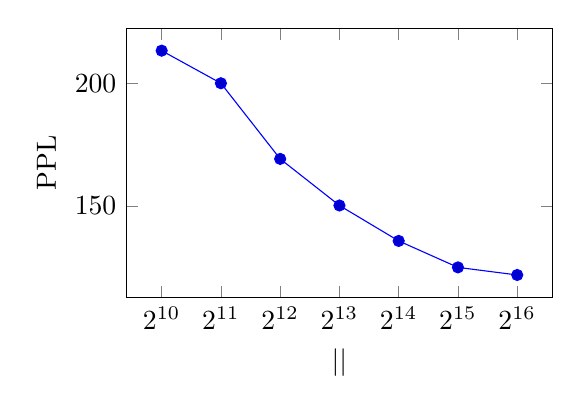
\begin{tikzpicture}
\begin{axis}[
    xlabel=$|\mcZ|$,
    ylabel=PPL,
    xmode=log,
    log basis x={2},
    xtick={},
    width=7cm,
    height=5cm
]
  \addplot plot coordinates {
    (1024,  213.25)
    (2048,  199.98)
    (4096,  169.18)
    (8192,  150.22)
    (16384, 135.79)
    (32768, 125.02)
    (65536, 121.93)
};
\end{axis}
\end{tikzpicture}
\caption{\label{tbl:states-ablation}
Perplexity on \texttt{PTB} by state size $|\mcZ|$ ($\lambda =0.5$ and $M=128$).
}
\end{figure}


\begin{table}[!t]
\centering
\begin{tabular}{llrrr}
\toprule
Model                & Param & Train  & Val  &  Time \\
\midrule
VLNHMM ($2^{14}$)    & 7.2M & 115    & 134  & 40\\
\quad - neural param & 423M & 119    & 169  & 14\\
\quad - dropout      & 7.2M & 88     & 157  & 100\\
\bottomrule
\end{tabular}
\caption{\label{tbl:dropout-param-ablation}
Ablations on \texttt{PTB} ($\lambda =0.5$ and $M=128$). 
Time is ms per eval batch (Run on RTX 2080).
}
\end{table}


\section{Conclusion}
This work demonstrates that scaling HMMs to large states spaces results in performance gains.
In order to scale, we introduce three techniques:
a blocked emission constraint, a neural parameterization,
and state dropout, which lead to an HMM that outperforms n-gram models and prior HMMs.
Once scaled up to take advantage of modern hardware,
very large HMMs demonstrate meaningful improvements over smaller HMMs
and are worthy of consideration for NLP tasks. 

\section*{Acknowledgements}
We are grateful to
Yuntian Deng, Daniel Fried, Yao Fu, Yoon Kim, Victor Sanh, and Sam Wiseman
for insightful conversations and suggestions.

\bibliographystyle{acl_natbib}
\bibliography{anthology,emnlp2020}

%\clearpage
\appendix

\section{Appendices}
\subsection{Inference and Learning in HMMs}
In this section we review the computation of the evidence of observed words $p(\bx)$ in an HMM.
Recall that the evidence is given by
\begin{equation}
\begin{aligned}
p(\bx) &= \sum_\bz p(\bx, \bz)\\
&= \sum_{\bz} \prod_{t=1}^T p(z_t \mid z_{t-1})p(x_t \mid z_t) \\
&= \sum_{z_1} \cdots \sum_{z_T} p(z_1 \mid z_0)p(x_1 \mid z_1)\\
&\qquad \cdots p(z_T \mid z_{T-1})p(x_t \mid z_T)
\end{aligned}
\end{equation}
where $p(z_0=\epsilon)=1$ is a dummy state for ease of notation.
Now consider matrices $\bF_t$ with
elements $F_{ij} = p(z_t = j \mid z_{t-1} = i) p(x_t \mid z_t = j)$.
Note that $\mathbf{f}_1 \in \R^{|\mcZ|}$ since there is only a single starting state $z_0 = \epsilon$,
while $\bF_t \in \R^{|\mcZ|\times|\mcZ|}$ for $t \in [2, \ldots, T]$.
Repeated application of the distributive rule allows us to express the above in 
matrix notation
\begin{equation}
\label{eqn:mat_ev}
p(\bx) = \mathbf{f}_1^T \bF_2 \cdots \bF_{T-1}\bF_{T}\mathbf{1}
\end{equation}
where $\mathbf{1}$ is a column vector with all entries equal to 1.
In this form the runtime is explicit: there are $O(T)$ matrix-vector products
resulting in $O(T |\mcZ|^2)$ computation.\footnote{
One can apply the associative property of matrix multiplication
to perform Eqn.~\ref{eqn:mat_ev} as a binary tree reduction,
resulting in $O(\log(T)|\mcZ|^3)$ runtime on a parallel machine.
}
Additionally, computing gradients with respect to each $\bF_t$ can be done with
any automatic differentiation library, as all operations in Eqn.~\ref{eqn:mat_ev} are differentiable.

Block-sparse emissions and state dropout serve to zero out entries of each $\bF_t$,
allowing us to only consider dense submatrices of each matrix $\bF_t$ in Eqn.~\ref{eqn:mat_ev}.

\subsection{Brown Clustering}
TODO: finish

\subsection{Hyperparameters}
\label{sec:hyperparams}

For \texttt{Penn Treebank} and \texttt{Wikitext-2}, we trained the following baselines:
a two layer FF 256-dim 5-gram model and a two layer 256-dim LSTM.
The FF model is given by the following:
\begin{equation}
\begin{aligned}
p(w_t \mid \bw_{<t})
&= W_x\textrm{ReLU}(\textrm{Conv}(\mathbf{E}_w(\bw_{t-4:t-1})))
\end{aligned}
\end{equation}
where $\mathbf{E}_w$ gives the word embeddings and
$W_x\in\mathbb{R}^{|\mcX|\times h}$ is weight-tied to the embeddings.

For the (5-gram) FF model we use a batch size of 128 and a bptt length of 64,
as we found the model needed a larger batch size to achieve decent performance.
For the LSTM, we use a batch size of 16 and a BPTT length of 32.
For both baseline models we use AdamW \citep{adamw} with a learning rate of 1e-3 and a dropout rate of 0.3 on the activations in the model.
Both models use a hidden dimension of 256 throughout.
These same hyperparameters were applied on both \texttt{Penn Treebank} and \texttt{Wikitext-2}.

For the HMMs we use a batch size of 16 and a BPTT length of 32.
We use state dropout with rate $\lambda = 0.5$.
We use AdamW \citep{adamw} with a learning rate of 1e-2 for \texttt{Penn Treebank},
and a learning rate of 1e-3 for \texttt{Wikitext-2}.

All weights are initialized with the Kaiming uniform initialization.
The FF model was trained for 100 epochs, while all other models were trained for 50.
Validation likelihood was checked 4 times per epoch, and
learning rates were decayed by a factor of 4 if the validation performance
did not improve after 8 checks.

Hyperparameter search was performed manually, using the best
validation perplexity achieved in a run.
Bounds:
\begin{enumerate}
\item Learning rate $\in \set{0.0001, 0.001, 0.01, 0.1}$
\item Dropout $\lambda \in \set{0, 0.25, 0.5, 0.75}$
\item Hidden dimension $h \in \set{128,256,512}$
\item Batch size $\in \set{16, 32, 64, 128}$
\end{enumerate}

Experiments were run on RTX 2080 GPUs.

On \texttt{PTB} the FF model takes 3s per epoch, the LSTM 23s,
and the VLHMM $2^{15}$ 433s.
The inference for VLHMM was not heavily optimized,
and uses a kernel produced by TVM \citep{tvm} for computing
gradients through marginal inference.

\subsection{HMM Parameterization}
Let $\mathbf{E},\mathbf{D}\in\mathbb{R}^{v \times h}$ be an
embedding matrix and a matrix of the same size,
where $v$ is the size of the vocab and $h$ the hidden dimension.
We use the following residual network as our MLP:
\begin{equation}
\label{eqn:res}
\begin{aligned}
f_i(\mathbf{E}) &= g_i(\textrm{ReLU}(\mathbf{E}W_{i1}))\\
g_i(\mathbf{D}) &= \textrm{LayerNorm}(\textrm{ReLU}(\mathbf{D}W_{i2}) + \mathbf{D})
\end{aligned}
\end{equation}
with $i \in \set{\textrm{out},\textrm{in},\textrm{emit}}$,
$W_{i1},W_{i2} \in \mathbb{R}^{h \times h}$.
The state embeddings are then obtained by
\begin{equation}
\begin{aligned}
\mathbf{H}_\textrm{out} &= f_\textrm{out}(\mathbf{E}_z)\\
\mathbf{H}_\textrm{in} &= f_\textrm{in}(\mathbf{E}_z])\\
\mathbf{H}_\textrm{emit} &= f_\textrm{emit}(\mathbf{E}_m,\mathbf{E}_z)
\end{aligned}
\end{equation}

We additionally experiment with factored state embeddings.
TODO: finish.
We introduce residual networks $f_j,j\in\set{o,i,e}$
to compose block and state embeddings, yielding
\begin{equation}
\begin{aligned}
\mathbf{H}_\textrm{out} &= f_\textrm{out}(f_o([\mathbf{E}_m,\mathbf{E}_z]))\\
\mathbf{H}_\textrm{in} &= f_\textrm{in}(f_i([\mathbf{E}_m,\mathbf{E}_z]))\\
\mathbf{H}_\textrm{emit} &= f_\textrm{emit}(f_e([\mathbf{E}_m,\mathbf{E}_z]))
\end{aligned}
\end{equation}

\begin{table}[t]
\centering
\begin{tabular}{lllll}
\toprule
Constraint & $|\mcZ|$ & $|\mcC_x|$ & $m$ & Val PPL\\
\midrule
Brown & 16384 & 512 & 32  & 137\\
Brown & 16384 & 256 & 64  & 138\\
Brown & 16384 & 128 & 128 & 134\\
Brown & 16384 & 64  & 256 & 136\\
\midrule
None  & 1024 & - & - & 180\\
Brown & 1024 & 256 & 4 & 182\\
Brown & 1024 & 128 & 8 & 194\\
\midrule
Uniform    & 8192    & 128    & -   & 150\\
Brown      & 8192    & 128    & 64  & 142\\
Uniform    & 16384   & 128    & -   & 146\\
Brown      & 16384   & 128    & 128 & 136\\
\bottomrule
\end{tabular}
\caption{\label{tbl:constraint-ablation}
Emission constraint ablations on \texttt{Penn Treebank}.
}
\end{table}


\subsection{Emission Constraint Ablation}
Tbl.~\ref{tbl:constraint-ablation} shows the results from 
emission constraint ablations.
For the ablations in this section,
we do not use the factored state embedding
and instead directly learn embeddings $\mathbf{E}_z\in\mathbb{R}^{|\mcZ|\times h}$.
We examine the effect of factored state embeddings in the next section.

With a VLNHMM that has $|\mcZ|=2^{14}$ states,
the model is insensitive to the number of blocks $M$.
However, with fewer states $|\mcZ|=2^{10}$ where we are able to
able to use fewer blocks to examine whether the block-sparsity
of the emission results in a performance loss.
With $M=4$ blocks, the block-sparse HMM matches an unconstrained HMM
with the same number of states.
When $M=8$, the block-sparse model underperforms,
implying there may be room for improvement with the larger
HMMs that use $M > 8$ blocks.

We additionally compare the blocks induced by Brown clustering with a uniform
constraint that samples subsets of states of size $n$
independently and uniformly from $\mcZ$.
This does not admit a partitioning, which makes it difficult to apply state dropout.
We therefore zero out half of the logits of the transition matrix randomly
before normalization.
In the bottom of Tbl.~\ref{tbl:constraint-ablation},
we find that models with uniform constraints
are consistently outperformed by models with Brown cluster constraints
as measured by validation perplexity.
The models with uniform constraints also had poor validation performance
despite better training performance, a symptom of overfitting.

These ablations demonstrate that the constraints based on
Brown clusters used in this work may not be optimal,
motivating future work that learns sparsity structure.

\subsection{Factored State Representation Ablation}
We examine the effect of factoring state representations into block embeddings
and independent state embeddings.
Recall that factored state representations were parameterized via 
\[ \mathbf{H}_{\textrm{out}},\mathbf{H}_{\textrm{in}},\mathbf{H}_\textrm{emit}
 = \text{MLP}(\mathbf{E}_m, \mathbf{E}_z ) \] 
with the block and state embeddings 
$\mathbf{E}_m,\mathbf{E}_z \in \mathbb{R}^{|\mcZ| \times h/2}$).
We ablate this by comparing to the following independent state representation:
\[ \mathbf{H}_{\textrm{out}},\mathbf{H}_{\textrm{in}},\mathbf{H}_\textrm{emit}
 = \mathbf{E}_z' \] 
with $\mathbf{E_z'}\in\mathbb{R}^{|\mcZ| \times h}$.
The results of the factored state ablation are in Fig.~\ref{fig:fac-ablation},

We find that the performance of independent state embeddings with
is similar to a model with factored embeddings,
until the number of blocks is $\le 64$.

\begin{figure}[h]
\centering
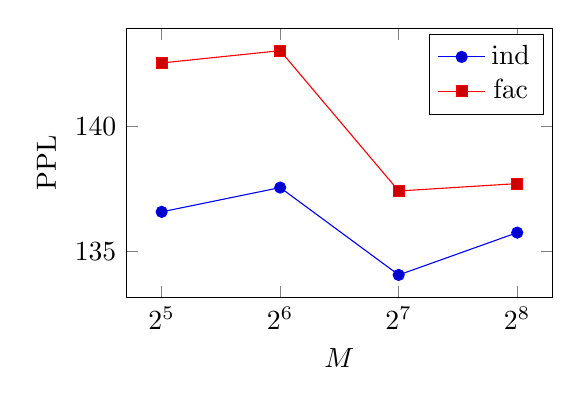
\begin{tikzpicture}
\begin{axis}[
    xlabel=$M$,
    ylabel=PPL,
    xmode=log,
    log basis x={2},
    xtick={},
    width=7cm,
    height=5cm
]
  \addplot plot coordinates {
    (32,  136.58)
    (64,  137.55)
    (128, 134.06)
    (256, 135.75)
  };
  \addlegendentry{ind}
  \addplot plot coordinates {
    (32,  142.528)
    (64,  143.02)
    (128, 137.415)
    (256, 137.708)
  };
  \addlegendentry{fac}
\end{axis}
\end{tikzpicture}
\caption{\label{fig:fac-ablation}
Perplexity on \texttt{PTB} by number of blocks $M$ ($\lambda =0.5$ and $|\mcZ|=2^{14}$).
}
\end{figure}

\subsection{Computational Considerations}

\begin{table}[h]
\centering
\begin{tabular}{llrrr}
\toprule
Model                & Size & Train  & Val & Time \\
\midrule
VLNHMM ($2^{14}$)    & 7.2M & 115    & 134 & 40\\
\quad - neural param & 423M & 119    & 169 & 14\\
\quad - dropout      & 7.2M & 88     & 157 & 100\\
\quad + block emb    & 5.6M & 122    & 136 & 48\\
\bottomrule
\end{tabular}
\caption{\label{tbl:dropout-param-ablation-repeat}
Ablations on \texttt{PTB} ($\lambda =0.5$ and $M=128$). 
Time is ms per eval batch (Run on RTX 2080).
}
\end{table}

We reproduce the technique ablation table here in
Tbl.~\ref{tbl:dropout-param-ablation-repeat} for reference.
As we remove neural components, 
the number of parameters increases but the time of the
forward pass decreases.
This is because generating parameters from a neural network
takes strictly more time than having those parameters available,
similar to a hierarchical Bayesian model.

When block embeddings are removed and the state representations are
directly parameterized,
the model is faster due to not needing to recompute state representations.
This contrast is even more pronounced when removing neural components altogether,
with an almost 3x speedup.
However, we note that the drop in generalization is large,
indicating the neural parameterization helps with learning.
Therefore we use the neural parameterization at training time,
then cache the resulting HMM parameters (the transition and emission matrices)
for use during inference.

\end{document}
